\documentclass[aspectratio=169]{beamer}
\usetheme{default}
\usecolortheme[dark]{solarized}

\usepackage{minted}
\usemintedstyle{solarizeddark}

\usepackage[english]{babel}

\usepackage[utf8]{inputenc}

\usepackage{times}
\usepackage[T1]{fontenc}

\newcommand{\alerturl}[1]{\alert{\url{#1}}}

\title{Live Traffic Information with Python}
\author{Rich Wareham}

\institute{%
  Department of Engineering\\
  University of Cambridge
}

\date{29 April 2013}

\subject{Talks}

\newcommand{\tallimage}[1]{%
  \begin{frame}
    \centering
    \includegraphics[height=0.95\textheight]{#1}
    \\
  \end{frame}
}

\newcommand{\wideimage}[1]{%
  \begin{frame}
    \centering
    \includegraphics[width=\textwidth]{#1}
    \\
  \end{frame}
}

\begin{document}

\section{Title}

\begin{frame}
  \titlepage
\end{frame}

\section{Introduction}

\tallimage{img/nasa-mission-control.jpg}
\wideimage{img/norad.jpg}
\wideimage{img/wargames.png}
\begin{frame}
  \centering\Large
  \url{http://rjw57.github.io/proj4webgl/}
  \\
  \vspace{\baselineskip}
  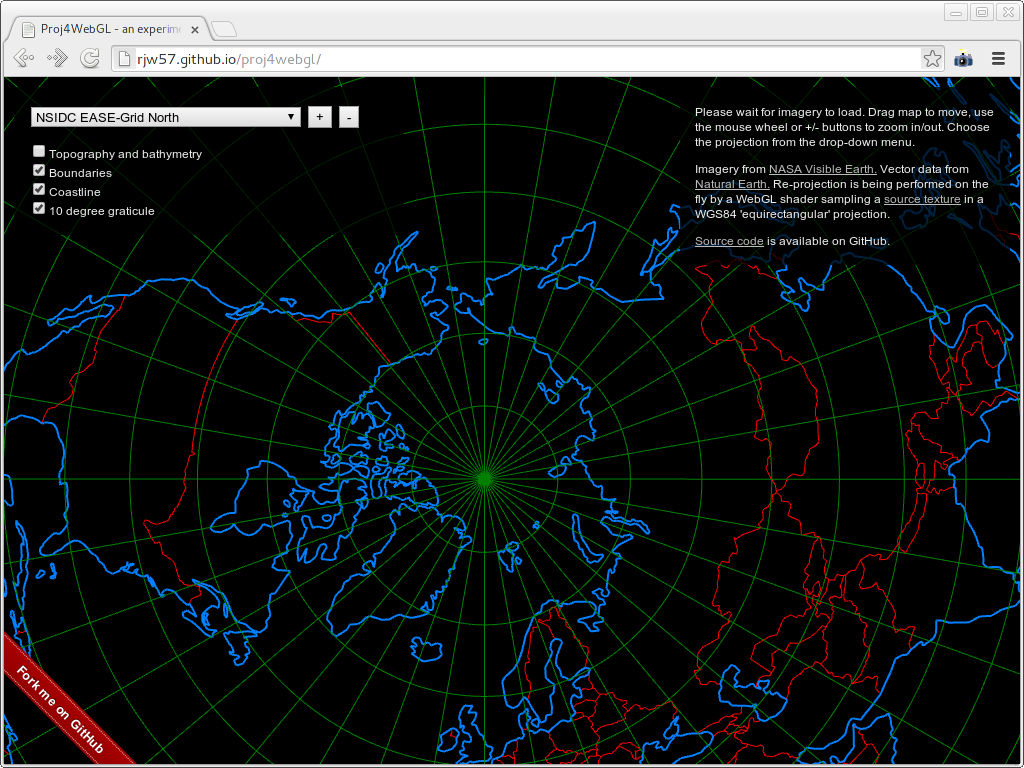
\includegraphics[height=0.8\textheight]{img/proj4webgl.png}
  \\
\end{frame}
\wideimage{img/norad.jpg}
\tallimage{img/control-centre.jpg}
\tallimage{img/highways-agency-logo.jpg}
\tallimage{img/network-map.png}
\tallimage{img/control-screen.jpg}
\wideimage{img/wargames.png}
\tallimage{img/cambridge-traffic-data.png}

\begin{frame}
  \Huge\centering
  \url{http://data.gov.uk/}
  \\
\end{frame}

\tallimage{img/data-gov-uk.png}
\tallimage{img/data-page.png}
\wideimage{img/data-page-crop.png}

\begin{frame}
  \Large\centering
  \url{http://hatrafficinfo.dft.gov.uk/feeds/datex/England/}\alerturl{PredefinedLocationLinks}\url{/content.xml}
  \\
  \vspace{1\baselineskip}
  \url{http://hatrafficinfo.dft.gov.uk/feeds/datex/England/}\alerturl{TrafficData}/\url{content.xml}
  \\
\end{frame}

\tallimage{img/datex2.png}

\section{Link data}

\subsection{Parsing with LXML}
\begin{frame}
  \inputminted{xml}{document.xml}
  \vspace{\baselineskip}
  \inputminted{python}{lxml_objectify.py}
\end{frame}

\subsection{Parsing Link data}
\begin{frame}
  \centering\Huge
  PredefinedLocationLinks
  \\
\end{frame}

\begin{frame}
  \inputminted{xml}{PredefinedLocationLinks/structure.xml}
\end{frame}

\begin{frame}
  \inputminted{xml}{PredefinedLocationLinks/location.xml}
\end{frame}

\begin{frame}
  \inputminted{python}{PredefinedLocationLinks/structure.py}
\end{frame}

\begin{frame}
  \inputminted{python}{PredefinedLocationLinks/structure_out.py}
\end{frame}

\begin{frame}
  \inputminted{python}{wgs84-links.py}
\end{frame}

\wideimage{img/wgs84-links.pdf}

\begin{frame}
  \inputminted[lastline=7]{python}{bng-links.py}
\end{frame}

\begin{frame}
  \inputminted[firstline=9, lastline=19]{python}{bng-links.py}
\end{frame}

\begin{frame}
  \inputminted[firstline=21, lastline=31]{python}{bng-links.py}
\end{frame}

\wideimage{img/bng-links.pdf}

\begin{frame}
  \centering
  \parbox{0.6\textwidth}{%
    \url{https://github.com/rjw57/foldbeam/}
    \\
    \vspace{2\baselineskip}
    \inputminted{console}{foldbeam-render.sh}
  }
  \\
\end{frame}

\begin{frame}
  \inputminted[firstline=33, lastline=40]{python}{bng-links.py}
\end{frame}

\wideimage{img/bng-links-2.pdf}

\section{Traffic Data}

\begin{frame}
  \centering\Huge
  TrafficData
  \\
\end{frame}

\begin{frame}
  \inputminted{xml}{TrafficData/content.xml}
\end{frame}

\begin{frame}
  \inputminted{python}{TrafficData/parse.py}
\end{frame}

\begin{frame}
  \inputminted{python}{TrafficData/link_data.py}
\end{frame}

\begin{frame}
  \inputminted{python}{TrafficData/hist.py}
\end{frame}

\begin{frame}
  \centering\Huge
  Movie
  \\
\end{frame}

\tallimage{img/git-repo.png}

\begin{frame}
  \inputminted{python}{bng-speed-links.py}
\end{frame}

\begin{frame}
  \centering\Huge
  Movie
  \\
\end{frame}

\begin{frame}
  \inputminted{python}{ephem.py}
\end{frame}

\section{Conclusions}

\begin{frame}{Conclusions}
  \begin{itemize}
    \item Python is a universal `glue' language.
    \item The IPython web notebook is amazing.
    \item Plotting and numerical processing on a par with MATLAB.
    \item GPU acceleration is easily exposed as needed by PyOpenCL.
    \item Playing with data is fun.
    \item You too can make `mission control'.
  \end{itemize}
  \vspace{2\baselineskip}
  \begin{centering}
    \url{http://gplus.to/richwareham} $\quad$ \url{rjw57@cam.ac.uk}\\
  \end{centering}
\end{frame}

\end{document}

% vim:sw=2:sts=2:et
